\chapter{User Manual}
This appendix will provide instructions on how to bring the proxy up and how to operate each of the project's modules.
\section{Blockchain}
For simplicity, this guide will be using Blockchain network created through Ganache. It is not essential and any other Ethereum node can be used, which should be accessible via TCP connection.

To install Ganache, please follow instructions on https://www.trufflesuite.com/ganache to download AppImage and execute it from command line, like shown in listing \ref{cap:gan}. This should bring up interface similar as shown on figure \ref{fig:ganache}. Take note of the top two accounts, we will be using them in further examples.

\begin{lstlisting}[language=bash,breaklines=true,label={cap:gan},caption={Launching Ganache}]
$ chmod +x ganache-2.3.1-linux-x86_64.AppImage
$ ./ganache-2.3.1-linux-x86_64.AppImage
\end{lstlisting}

You can click on the key icon on the far right in order to retrieve account's private key. I recommend saving the first one as `privkey.asc' and the second one as `clientPriv.asc'. Those will be our private keys used in further examples.
\section{MQTT Broker}
We will be using HiveMQ test broker located under broker.hivemq.com:1883, so you don't need a local instance on your machine. HiveMQ doesn't support TLS connections, so all examples will have tls flag set to false, though if desired, it can be set to true, as long as the target support TLS and provides a certificate.
\section{Parameters}
\subsection{Common env variables}\label{sec:envvars}
FlyTrap and Blockchain CLI makes use of two environmental variables. It is very important to set them before performing any action:
\begin{description}
  \item[FLYTRAP\_CONTRACT] - public address of FlyTrap's smart contract. You will not know it until you run blockchain CLI with -new flag. Once you obtain it, it's recommended to update this variable.
  \item[BLOCKCHAIN\_ADRRESS] - endpoint to access Ethereum node. For Ganache, default is http://localhost:7545.
\end{description}
I recommend to put the following two lines in your .bashrc file (or corresponding rc file, if your shell is different than bash):
\begin{lstlisting}[language=bash,breaklines=true]
export BLOCKCHAIN_ADDRESS="http://localhost:7545"
export FLYTRAP_CONTRACT="<contract address>"
\end{lstlisting}
\subsection{Flytrap}
\begin{lstlisting}[language=bash,breaklines=true]
$ go build -o flytrap cmd/flytrap/main.go
$ ./flytrap -help
Usage of ./flytrap:
  -b string
    	Provide address of MQTT Broker. (default "test.mosquitto.org:8883")
  -bcrt string
    	location of broker's cert for TLS connection (default "broker.crt")
  -crt string
    	Location of your server's .crt used for TLS connection (default "server.crt")
  -freq duration
    	How often usage summaries should be saved on blockchain (default 30s)
  -key string
    	Location of your server's .key file used for TLS connection (default "server.key")
  -p string
    	Port to use for proxy server (default ":8888")
  -tls
    	Whether the proxy should be encrypted on both sides. You will need to provide .crt and .key files if so. (default true)
\end{lstlisting}
\paragraph{IMPORTANT} You need to set BLOCKCHAIN\_ADDRESS and FLYTRAP\_CONTRACT environmental variables, as they are used to determine respectively address of blockchain node to connect to and address of FlyTrap's contract on blockchain where the ACL rules are located at. 
\subsection{Blockchain}
\begin{lstlisting}[language=bash,breaklines=true]
$ go build -o blockchain cmd/blockchain/main.go
$ ./blockchain -help
Usage of ./blockchain:
  -client string
    	Public key of client to manipulate
  -contract string
    	Specify address of your contract
  -country string
    	topic will only be accessible to people connecting from this country. 2 letter ISO code. (default "GB")
  -date string
    	Provide date that should be searched for. E.g. 2020-02-29
  -logs
    	Receive relevant event logs. Providing -client and -topic flags will restrict the search only to relevant fields.
  -new
    	Whether to create new contract for flytrap
  -new_topic string
    	Reason to create a new topic
  -pub string
    	Reason to add as publisher
  -pub_cost int
    	cost of adding as publisher in wei
  -rpub string
    	Reason to revoke as publisher
  -rsub string
    	Reason to revoke as subscriber
  -s	whether new topic is to be marked as sensitive (default true)
  -sub string
    	Reason to add as subscriber
  -sub_cost int
    	cost of adding as subscriber in wei
  -topic string
    	name of the topic to modify (default "MyTopic1")
  -v	Enable verbose mode
\end{lstlisting}
\paragraph{IMPORTANT} You need to set BLOCKCHAIN\_ADDRESS and FLYTRAP\_CONTRACT environmental variables, as they are used to determine respectively address of blockchain node to connect to and address of FlyTrap's contract on blockchain. Those values are needed to run any commands (except creating new contract, for that only the former is required).
\subsection{MQTT Client}
This binary is used to use MQTT requests towards the broker. Please note, you should place clientPriv.asc file that you obtained from Ganache and place it adjacent to the binary. During execution, the client will produce an extra pub\_clientPriv.asc and sig\_clientPriv.asc files which serve as cache to avoid repeated signature calculations. 
\begin{lstlisting}[language=bash,breaklines=true]
$ go build mqttclient/client.go
$ ./client -help
Usage of ./client:
  -conn_test
    	whether to only connect and then immediately disconnect
  -crt string
    	location of cert for SSL/TLS connection (default "flytrap.crt")
  -f	Whether to force recomputation of signature
  -id string
    	ID of connecting client
  -ip string
    	location of MQTT broker (default "localhost:8888")
  -msg string
    	message to be published (default "Here Be Dragons")
  -priv string
    	Location of your private key file (default "privkey1.asc")
  -pub int
    	How many messages to publish
  -sub int
    	How many messages to receive via subscription
  -tls
    	whether to use TLS (default true)
  -topic string
    	Topic for use for pub/sub (default "MyTopic1")
\end{lstlisting}
\subsection{WebApp}
WebApp doesn't offer any command line parameters and by default will run on port :8081. If you would like to change this to something else, you can edit the constant in Line 14 of webapp/main.go file.

FLYTRAP\_CONTRACT is an optional env variable. If set, the contract field will be pre-populated when website is rendered. Otherwise, it will remain blank.
\section{Usage Examples}
This section will walk you through how to use each of the modules to perform all functionality offered by FlyTrap.
\subsection{Blockchain}
Operations described in this section will demonstrate how to manipulate and interact with FlyTrap's smart contract located on Ethereum. Before running any of those examples, make sure you have configured your env variables as per section \ref{sec:envvars}.

\paragraph{IMPORTAT} Make sure privkey.asc is in the same directory from where you execute the go run commands.
\subsubsection{Creating a new contract}
This operation will create a new contract on Blockchain and output its public key. Make sure your account has enough funds, as it might cost some gas.
\begin{lstlisting}[language=bash,breaklines=true]
$ go run cmd/blockchain/main.go -new -contract=""
2020/04/20 18:02:37 Generated new contract, address is: 0x278AC0391ceA1E7664D4242C7398FCDe79539a93
\end{lstlisting}
I \textbf{strongly} recommend to save the obtained address in environmental variable as per section \ref{sec:envvars}.
\subsubsection{Creating a new topic}
This operation will create a new topic on FlyTrap's contract.
\begin{lstlisting}[language=bash,breaklines=true]
$ go run cmd/blockchain/main.go -new_topic="reason to create topic" -topic="MyTestingTopic" -pub_cost=0 -sub_cost=0
\end{lstlisting}
As a -new\_topic param you need to provide a reason to create a new topic, along with -topic flag to specify its name. If pub cost and sub cost is set to 0, then only topic's owner can alter its state. Otherwise, anyone can do it, provided they pay required amount (which would be transferred to the original owner)
\subsubsection{Adding subscribers/publishers}
\begin{lstlisting}[language=bash,breaklines=true]
$ go run cmd/blockchain/main.go -topic="MyTestingTopic" -client="<client_pubkey>" -pub="Addining a new publisher"
\end{lstlisting}
Under -client flag, you can provide corresponding pubkey, as obtained from Ganache. This will allow it publish to MyTestingTopic. To add as a subscriber, change flag pub to sub.
\subsubsection{Revoking subscribers/publishers}
\begin{lstlisting}[language=bash,breaklines=true]
$ go run cmd/blockchain/main.go -topic="MyTestingTopic" -client="<client_pubkey>" -rpub="Revoking publisher"
\end{lstlisting}
Similar to adding, with the only exception that pub/sub flag is changed to rpub/rsub. This command will undo the addition and forbid specified client from further interaction with MyTestingTopic.
\subsection{FlyTrap}
This section will explain how to bring up your own FlyTrap proxy and connect it to HiveMQ test broker.
\subsubsection{Starting up FlyTrap}
\paragraph{IMPORTAT} Make sure privkey.asc is in the same directory as FlyTrap and BLOCKCHAIN\_ADDRES \& FLYTRPAP\_CONTRACT environmental are set and active. You can verify it by running `\$ echo \$BLOCKCHAIN\_ADDRESS \$FLYTRAP\_CONTRACT'. If you can see both values output to the terminal, you are ready to go.
\begin{lstlisting}[language=bash,breaklines=true]
$ echo $BLOCKCHAIN_ADDRESS $FLYTRAP_CONTRACT
http://localhost:7545 0x61c4603936627946aAb47a86e135b983171eFF44
$ go run cmd/flytrap/main.go -b="broker.hivemq.com:1883" -tls=false -freq=24h -p ":7777"
2020/04/20 18:26:12 Now accepting connections under :7777
\end{lstlisting}
This will initiate proxy under port :7777, generating reports for sensitive topics every 24hrs and connecting to MQTT broker located under broker.hivemq.com:1883. I recommend to minimize this window and move forward to the next section explaining how to submit messages through FlyTrap.
\subsection{MQTT Client}
This section will explain how to use provided MQTT client to subscribe and publish your own messages. 

\paragraph{IMPORTANT} For those tests, make sure that the private key clientPriv.asc that you obtained from Ganache is in your working directory.
\paragraph{NOTE} This client can also be used for any other MQTT Broker, i.e. -ip parameter can either point to FlyTrap or directly to the Broker (e.g. broker.hivemq.com:1883)
\subsubsection{Publishing}
\begin{lstlisting}[language=bash,breaklines=true]
$ go run client.go -pub=3 -topic="MyTestingTopic" -priv="clientPriv.asc" -ip="localhost:7777" -tls=false -f
2020/04/20 18:42:43 Published message: Here Be Dragons #0
2020/04/20 18:42:43 Published message: Here Be Dragons #1
2020/04/20 18:42:43 Published message: Here Be Dragons #2
2020/04/20 18:42:43 Published 3 messages, as requested, disconnecting
\end{lstlisting}
Command above will publish three messages to the topic MyTestingTopic under a broker located on localhost:7777 (where FlyTrap is currently running). We also specified the exact location of our private key and disable TLS (as testing hivemq broker doesn't support it). -f flag is used to compute signature again, regardless whether it's cached or not.

We can also refer back to our FlyTrap terminal to inspect that the messages where indeed received and passed forward to the broker:
\begin{lstlisting}[language=bash,breaklines=true]
2020/04/20 18:42:42 Now accepting connections under :7777
2020/04/20 18:42:43 Starting new proxy connection ([::1]:54764 >> broker.hivemq.com:1883)
2020/04/20 18:42:43 Client "0x4514A540Cf6c81B482Ac88d0627d4F71e9363885" was authorised to publish to topic "MyTestingTopic"
2020/04/20 18:42:43 Client "0x4514A540Cf6c81B482Ac88d0627d4F71e9363885" was already authorised to publish to topic "MyTestingTopic"
2020/04/20 18:42:43 Client "0x4514A540Cf6c81B482Ac88d0627d4F71e9363885" was already authorised to publish to topic "MyTestingTopic"
2020/04/20 18:42:43 Proxy Connection terminated gracefully. ([::1]:54764 >> broker.hivemq.com:1883)
\end{lstlisting}

\subsubsection{Subscribing}
\begin{lstlisting}[language=bash,breaklines=true]
$ go run client.go -sub=3 -topic="MyTestingTopic" -priv="privkey1.asc" -ip="localhost:7777" -tls=false -f
\end{lstlisting}
Subscribing works very similar to publishing, with the only exception that client will maintain connection until specified number of messages has been received (in this case, three) Again, we can see relevant runtime logs on FlyTrap's terminal window:
\begin{lstlisting}[language=bash,breaklines=true]
2020/04/20 18:46:35 Starting new proxy connection ([::1]:54824 >> broker.hivemq.com:1883)
2020/04/20 18:46:35 Client "0x4514A540Cf6c81B482Ac88d0627d4F71e9363885" was authorised to subscribe to topic "MyTestingTopic"
2020/04/20 18:50:05 Proxy Connection terminated gracefully. ([::1]:54824 >> broker.hivemq.com:1883)
\end{lstlisting}
\subsection{WebApp}
\paragraph{IMPORTANT} Make sure privkey.asc from Ganache is in your working directory.

Web application provides an extension to the project providing an easy overview of the data stored on blockchain. It queries the smart contract directly and does not require any of the remaining components to function. To start it, run the following command in your terminal:
\begin{lstlisting}[language=bash,breaklines=true]
$ go run main.go
2020/04/20 18:53:06 Server is now running under :8081
\end{lstlisting}

You can now navigate to http://localhost:8081 in a browser of your choice to access the application.
\subsubsection{Audits}
First tab is called `Audits' and contains information about all administrative actions taken on the given contract. The page will load empty (depending whether you set FLYTRAP\_CONTRACT variable, `Contracts Public Adress' might already by pre-populated). Enter the public address obtained when creating a new contract and time constraints. Please note, higher constraints might result in longer loadtime, so be sure to be as specific as possible.

\begin{figure}[h]
    \centering
    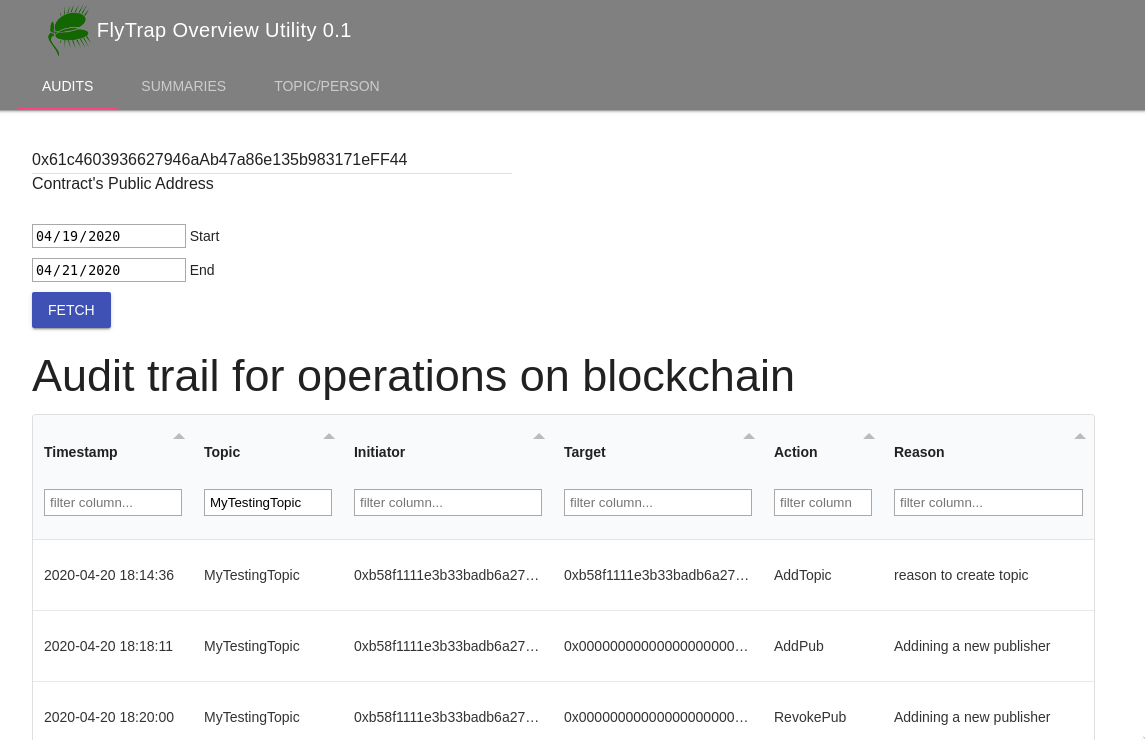
\includegraphics[width=\textwidth]{man1}
    \caption{Audits tab of the web application}
    \label{fig:man1}
\end{figure}
When finished loading, ``Audit trail for operations on blockchain'' table will be populated with the audit trail. It consists of six columns:
\begin{description}
 \item[Timestamp] - when the operation was performed
 \item[Topic] - affected topic
 \item[Initiator] - public key of the person initiating the operation
 \item[Target] - public key of the person affected by the change
 \item[Action] - what action was performed 
 \item[Reason] - reason provided by the initiator
\end{description}
The table can be then further filtered by filling the textboxes at the top of every column. In the example shown in figure \ref{fig:man1}, Topic column has been restricted only to actions containing MyTestingTopic. We can see the operations that were performed earlier in this manual.

The filters can be also further combined for even more precise search, e.g. to look up all AddPub events occurred on MyTestingTopic, we'd also fill the text box at Action column.
\subsubsection{Summaries}
This tab provides an overview of all logs registered on sensitive topics. As explained in section \ref{sec:reports}, their frequency relies on -freq field set when running FlyTrap.
\begin{figure}[h]
    \centering
    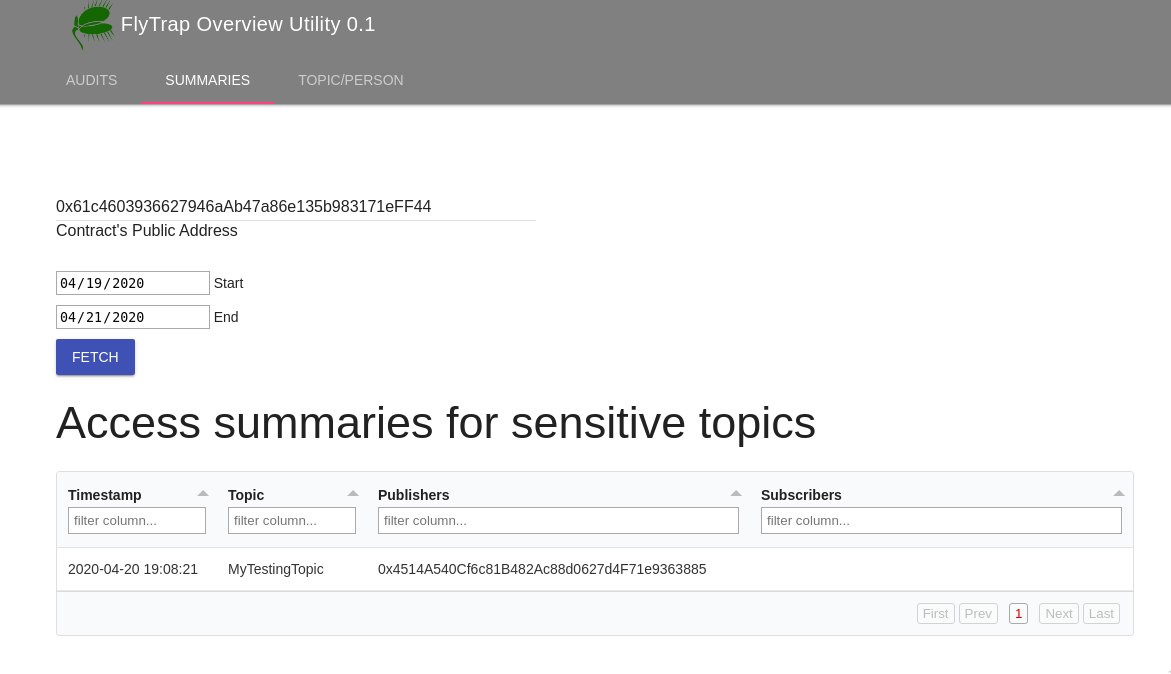
\includegraphics[width=\textwidth]{man2}
    \caption{Summaries tab of the web application}
    \label{fig:man2}
\end{figure}

Similar to Audits tab, we also need to fill the public address and time constraints. When ready, we can click ``Fetch'' which will populate the table, as shown in \ref{fig:man2}. This time, the table consists of 4 columns.
\begin{description}
  \item[Timestamp] - when the report was generated
  \item[Topic] - topic for which the report was generated
  \item[Publishers] - list of public keys that published to the given topic in the past X minutes from the specified Timestamp, where X is the frequency set in FlyTrap's command line parameters.
  \item[Subscribers] - similar as publishers, but for subscribers.
\end{description}
This table can also be further filtered, by using text boxes at the top of every column, to provide more precise records.
\subsubsection{Topic/Person}
This tab allows to look into the past and verify who had publishing/subscribing access to the given topic - or which topic given public key could publish/subscribe to. This is helpful for situation when a leak happens and you need to quickly determine who can access given resource, in order to revoke it.

Regardless whether we want to find out the first or the latter, we need to again fill the contract's public address along with a date. The results then will show access summaries at the end of specified day.

\begin{figure}[h]
    \centering
    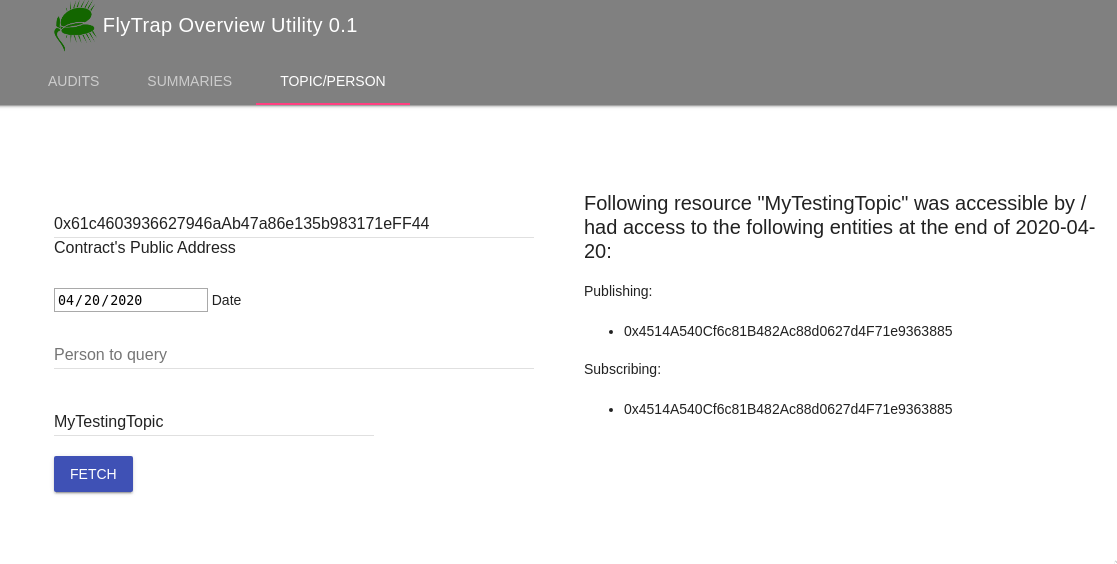
\includegraphics[width=\textwidth]{man3}
    \caption{Topic access summary}
    \label{fig:man3}
\end{figure}

As shown on figure \ref{fig:man3}, if we fill ``Topic to query'' text field, we we will obtain a result telling us that public key ``0x4514A540Cf6c81B482Ac88d0627d4F71e9363885'' was allowed to both publish and subscribe at the end of 2020-04-20.

\begin{figure}[h]
    \centering
    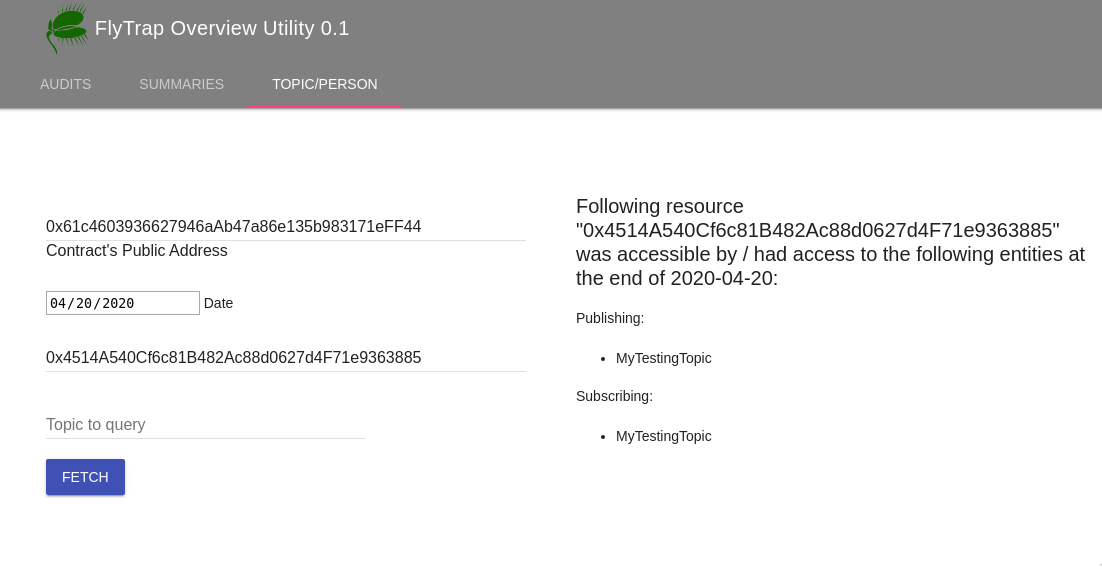
\includegraphics[width=\textwidth]{man4}
    \caption{Person access summary}
    \label{fig:man4}
\end{figure}

And if we fill ``Person to query'' text box - as per figure \ref{fig:man4}, we will find out that the given public key could both publish and subscribe to MyTestingTopic.
